% ACM TOG / SIGGRAPH methods draft. Build with `make` in this directory.
% Keep acmtog,anonymous,review for a Technical Papers submission.
% nonacm suppresses publication metadata for this unpublished working draft;
% remove it and enter the actual submission/rights metadata when submitting.
\documentclass[acmtog,anonymous,review,nonacm,pbalance]{acmart}

\citestyle{acmauthoryear}
\settopmatter{printacmref=false}
\setcopyright{none}
\acmJournal{TOG}
\acmDOI{}
\acmISBN{}
% \acmSubmissionID{actual submission ID}

\newcommand{\vect}[1]{\boldsymbol{#1}}
\newcommand{\norm}[1]{\lVert#1\rVert}
\newcommand{\pos}[1]{[#1]_{+}}
\newcommand{\cl}[1]{\textcolor{purple}{(CL: #1)}}
\newcommand{\red}[1]{\textcolor{red}{#1}}

\title[Two-Phase Flow with Melting Rigid Ice]{Two-Phase Flow with Melting Rigid Ice}
\subtitle{Method Draft}
% Author information is hidden by the anonymous class option.
% Add \author, \affiliation, and \email here for a non-anonymous version.

\begin{document}

% This compact document intentionally contains only the method.
% Add abstract, introduction, related work, results, and conclusions when
% extending it to a full paper; doing so changes the four-page budget.
\maketitle
% Source of truth: the current working-tree iceflow2d_v3 implementation.
% This describes the connected_ls / consistent_flux / cm_mrt / enthalpy_fv
% path used by the current dam-break examples, not every legacy option.
\section{Method}
\label{sec:method}

We couple a diffuse air--water interface to independently translating,
rotating, and eroding rigid ice bodies on a two-dimensional Cartesian grid. Fluid momentum
and phase evolve with a lattice Boltzmann method (LBM); water heat lives on
the spatial grid, while ice mass and heat remain on body-attached material
grids. This separation avoids transporting ice enthalpy through the fluid
grid during rigid motion. We use a \emph{disappearing-melt} approximation:
latent heat removes ice, without injecting liquid, heat, or momentum into
the surrounding fluid. The method therefore describes thermally driven
erosion with fluid--solid interaction, rather than a closed, mass-conserving
ice-to-water conversion.

\subsection{State and Discretization}
\label{sec:state}
% simulator.py: MovingBodyThermal2D, _sample_body_fraction,
% _reduce_moving_body_mass_properties, _apply_moving_body_mass_properties.
Let $h$ be the grid spacing, $t$ time, and $\Delta t$ the fluid time step. All flow
equations below use lattice units ($h=\Delta t=1$); the thermal equations
use physical units and unit out-of-plane thickness. At a fluid cell $x$,
we store phase $\phi_x\in[0,1]$ (air: 0; water: 1), pressure $p_x$,
velocity $\vect u_x$, and momentum and phase populations $f_q$ and $g_q$.
The two-dimensional, nine-velocity (D2Q9) lattice has directions
$q=0,\ldots,8$ with velocities $\vect c_q$; $q=0$ is rest.
Material subscripts $a,w,s$ label air, water, and ice, whose fixed
densities are $\rho_a,\rho_w,\rho_s$. Fluid density is
$\rho(\phi)=\rho_a+(\rho_w-\rho_a)\phi$, independently of pressure.
Each material cell $a$ stores surviving mass $m_a$, sensible energy $E_a$,
and surviving fraction $s_a=m_a/(\rho_s h^2)$. Bilinear interpolation under
the rigid transform gives spatial coverage $s(x)$; its $s=0.5$ isocontour
defines the impermeable ice boundary. Remaining mass determines the body
center and inertia, including the cell term $m_a s_a h^2/6$.

\subsection{Coupled Phase and Momentum Transport}
\label{sec:flow}
% lattice.py: momentum_equilibrium, phase_equilibrium.
% simulator.py: _collide_phase_kernel, _collide_momentum_kernel,
% _fluid_force_and_gradient, _prepare_capillary_stress, _update_pressure.
We use a conservative Allen--Cahn transport model
\citep{Geier2015}, with mobility $M$, interface width $W$, compression
strength $\lambda$, and regularized interface normal $\vect n_\epsilon$:
\begin{equation}
      \begin{aligned}
            \partial_t\phi+\nabla\!\cdot(\phi\vect u)
                             & =\nabla\!\cdot\left[M(\nabla\phi-\lambda\vect n_\epsilon)\right], \\
            \lambda=\frac{4\phi(1-\phi)}{W},\qquad
            \vect n_\epsilon & =\frac{\vect D}{\sqrt{\norm{\vect D}^2+\epsilon^2}}.
      \end{aligned}
      \label{eq:phase}
\end{equation}
Here $\vect D$ is the shared discrete phase gradient
(Section~\ref{sec:reconstruction}), $\epsilon>0$ is its normalization
regularizer, and $\norm{\cdot}$ is the Euclidean norm.
\red{Normal filtering can suppress bulk-phase
      artifacts \citep{Sato2023};} \cl{This seems new?} here we use the smooth normalization in
Eq.~\eqref{eq:phase}. D2Q9 quadrature weights are
$w_q=4/9$, $1/9$, and $1/36$ for rest, axial, and diagonal directions.
Following \citet{Liang2018}, define the velocity polynomial
$Q_q=3\vect c_q\!\cdot\vect u+
      \tfrac92(\vect c_q\!\cdot\vect u)^2-\tfrac32\norm{\vect u}^2$.
Equilibria (superscript $\mathrm{eq}$) and momentum/phase sources $S_q,R_q$ are
\begin{equation}
      \begin{aligned}
            f_q^{\mathrm{eq}} & =3(w_q-\delta_{q0})p'+w_q\rho Q_q,
                              & g_q^{\mathrm{eq}}                          & =w_q\phi(1+Q_q),                              \\
            S_q               & =3w_q\left[\vect c_q\!\cdot\vect F
                                           +\Delta\rho(\vect c_q\!\cdot\vect u)
                                           (\vect c_q\!\cdot\vect D)\right],
                              & R_q                                        & =w_q\lambda\vect c_q\!\cdot\vect n_\epsilon ,
      \end{aligned}
      \label{eq:equilibria}
\end{equation}
Here $\delta_{q0}$ is the Kronecker delta, $\Delta\rho=\rho_w-\rho_a$ is
the density contrast, $p'=p-p_0$ is dynamic pressure, and $\vect F$ is force
per unit lattice volume. The hydrostatic reference $p_0$ satisfies
$\partial_y p_0=\rho_0 g_y$ for fixed reference density $\rho_0$,
vertical coordinate $y$, and gravitational acceleration $\vect g$.
Trapezoidal integration constructs $p_0$; gravity contributes
$(\rho-\rho_0)\vect g$ to $\vect F$.
Thermal buoyancy adds
$-b(\phi)\rho_w\beta(T-T_{\mathrm{ref}})\vect g$, with
$b(\phi)=\max(0,2\phi-1)$ selecting water, $\beta$ its volume expansion
coefficient, and $T,T_{\mathrm{ref}}$ local and reference water temperatures.
For surface-tension coefficient $\sigma>0$, shared link tractions discretize
$\nabla\!\cdot\vect K$ using capillary stress
$\vect K=\tfrac32\sigma W
      (\norm{\vect D}^2\vect I-\vect D\vect D^{\mathsf T})$;
$\vect I$ is the identity and superscript $\mathsf T$ denotes transpose.

Pressure-based methods motivate central-moment multiple relaxation time
(MRT) collision \citep{Hajabdollahi2021}. We transform equilibria and sources
from Eq.~\eqref{eq:equilibria} together for basis consistency.
For either population set, the vector $\vect m$ of
central moments about $\vect u$ undergoes
\begin{equation}
      \vect m^\star=\vect m-\vect\Lambda(\vect m-\vect m^{\mathrm{eq}})
      +(\vect I-\tfrac12\vect\Lambda)\widehat{\vect S},
      \label{eq:collision}
\end{equation}
Here $\vect m^{\mathrm{eq}}$ contains equilibrium moments,
$\vect\Lambda$ is diagonal and contains relaxation rates, and
$\widehat{\vect S}$ contains transformed $S_q$ or $R_q$.
For LBM variables, stars denote post-collision, pre-streaming values.
The lattice kinematic viscosity is
$\nu=\phi\nu_w(T)+(1-\phi)\nu_a$, using converted water and air values.
Momentum shear modes relax at $(3\nu+1/2)^{-1}$; trace and fourth-order
modes share rate $0.25$, and the remaining modes relax at one.
This joint trace/fourth-order choice is specific to our pressure moments;
it adds acoustic damping independently of shear relaxation, motivated by
bulk/shear dissipation separation \citep{Qi2025}.
Phase first moments relax at $(3M+1/2)^{-1}$, higher moments at one,
and its zeroth moment is fixed to $\phi$.
% A rest-population correction closes this sum without changing transport moments.
After streaming,
\begin{equation}
      \begin{aligned}
            \phi & =\sum_q g_q,\qquad
            \vect u=\frac{\sum_q\vect c_q f_q+\vect F/2}{\rho},           \\
            p'   & =\frac35\left[\sum_{q\ne0}f_q
                                 +\frac12\Delta\rho\,\vect u\!\cdot\vect D
                                 -\frac23\rho\norm{\vect u}^2\right].
      \end{aligned}
      \label{eq:recovery}
\end{equation}
Out-of-range $\phi$ is clipped by lifting only the equilibrium part of
$g_q$.
% , followed by a rest correction.
Gradients are then recomputed before pressure recovery; valid phase values remain untouched.

% Queue the single-column method figure near the end of Sec. 1.2,
% allowing the figures to sit beside their Sec. 1.3 discussion.
\begin{figure}[t]
      \centering
      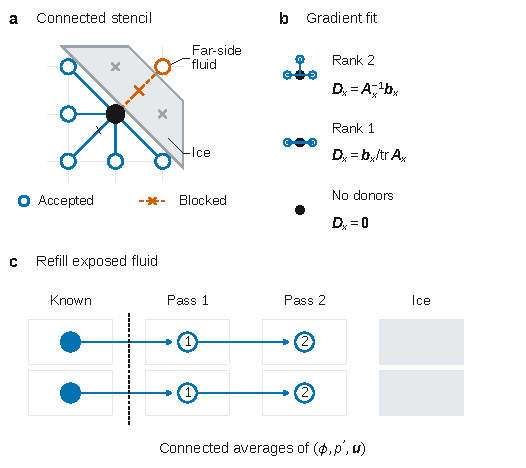
\includegraphics[width=\columnwidth]{figures/connected_reconstruction.pdf}
      \caption{Connected reconstruction. (a) The $3\times3$ stencil accepts
            connected donors and rejects ice or occluded samples.
            (b) Support rank selects the gradient solve: $\vect A_x,\vect b_x$
            are the normal matrix and right-hand side in
            Eq.~\eqref{eq:gradient}; $\operatorname{tr}$ denotes trace.
            (c) Known fluid seeds synchronous passes 1 and 2 for newly
            exposed cells. The dashed line marks the old ice edge;
            averages use states from the preceding pass.}
      \Description{A single-column diagram with connected-neighbor selection
            and rank-dependent gradient formulas above, and two rows of
            synchronous fluid-state propagation below. Blue circles indicate
            accepted donors; a dashed, crossed link marks an occluded sample.}
      \label{fig:reconstruction}
\end{figure}

% stability_options.py: _measure_phase_mass_flux, _phase_flux_force_density.
\paragraph{Mass--momentum consistency.}
Interface diffusion and compression in Eq.~\eqref{eq:phase} redistribute
mass beyond bulk advection. Omitting its momentum transport can generate
spurious velocity changes at large density ratios \citep{Mirjalili2021}.
With $\rho=\rho_a+\Delta\rho\phi$ and incompressibility
$\nabla\!\cdot\vect u=0$, multiplying Eq.~\eqref{eq:phase} by $\Delta\rho$
gives the continuum nonadvective mass flux $\vect J_{\mathrm c}$ and mass balance:
\begin{equation}
      \begin{aligned}
            \vect J_{\mathrm c}
             & =-\Delta\rho M(\nabla\phi-\lambda\vect n_\epsilon), \\
            \partial_t\rho+\nabla\!\cdot(\rho\vect u+\vect J_{\mathrm c})
             & =0.
      \end{aligned}
      \label{eq:mass-flux}
\end{equation}
Thus the total mass flux $\rho\vect u+\vect J_{\mathrm c}$ must transport
velocity as momentum per unit mass \citep{Mirjalili2021,Zhan2022}.
Its extra momentum flux is $\vect u\otimes\vect J_{\mathrm c}$, where
$\otimes$ denotes the outer product. Moving its divergence to the
right-hand side of the momentum equation gives a force containing both
$-\vect u(\nabla\!\cdot\vect J_{\mathrm c})$ and
$-(\vect J_{\mathrm c}\!\cdot\nabla)\vect u$ \citep{Zhan2022}.

To tie this correction to our phase collision, we estimate its flux from
the phase populations. Averaging their first moments before and after
collision and subtracting the advective flux $\phi\vect u$ isolates the
nonadvective contribution. We cache the pre-collision velocity $\vect u$,
collide phase, and use this same velocity to compute the discrete mass
flux $\vect J$ and its momentum force density $\vect F_J$:
\begin{equation}
      \begin{aligned}
            \vect J   & =\Delta\rho\left[\sum_q\vect c_q
                                         \frac{g_q+g_q^\star}{2}-\phi\vect u\right], \\
            \vect F_J & =-\nabla_h\!\cdot(\vect u\otimes\vect J).
      \end{aligned}
      \label{eq:flux}
\end{equation}
Here $\nabla_h$ is the discrete divergence. Across each open axial
face, arithmetic averages of $\vect J$ and the cached velocity form a
shared momentum flux with opposite contributions to adjacent cells;
closed faces carry no flux. We add $\vect F_J$ to $\vect F$ in both the
collision source and half-force recovery in
Eqs.~\eqref{eq:equilibria} and~\eqref{eq:recovery}. This explicit correction
adapts the consistent-transport principle to our existing pressure LBM.
% It does not establish exact consistency with individual streaming links
% or inherit discrete kinetic-energy conservation. Face limiting
% (Section~\ref{sec:scope}) further modifies the momentum correction without
% changing phase transport. This coupling accounts for redistribution of
% existing fluid mass; it supplies no meltwater source.

\begin{figure}[t]
      \centering
      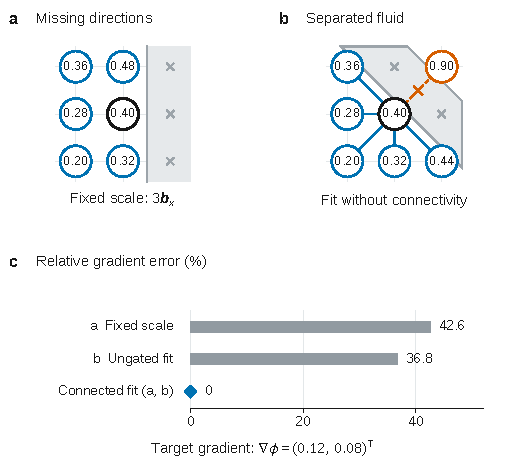
\includegraphics[width=\columnwidth]{figures/gradient_accuracy.pdf}
      \caption{Gradient accuracy for local affine data with
            $\nabla\phi=(0.12,0.08)^{\mathsf T}$ and $\phi_x=0.4$.
            Circle labels give phase values; gray regions are ice. (a) Fixed scaling
            $3\vect b_x$ uses accepted neighbors. (b) An ungated fit includes
            the independent sample $\phi=0.90$ across ice.
            (c) Relative error $100\norm{\vect D-\nabla\phi}/\norm{\nabla\phi}$,
            in exact arithmetic. Connected fits are rank two and exact;
            current single-precision kernel errors are below $3\times10^{-8}$.}
      \Description{Two local stencils above a horizontal error chart.
            Missing directions produce 42.6 percent error with fixed
            normalization; a separated fluid sample produces 36.8 percent
            error in an ungated fit. Connected fitting has zero analytic
            error in both cases. All quantities and labels are editable text.}
      \label{fig:gradient-accuracy}
\end{figure}

\subsection{Connected Derivatives and Newly Exposed Fluid}
\label{sec:reconstruction}
% phase_reconstruction.py: _prepare_phase_geometry,
% _prepare_phase_gradients_kernel, _refill_connected_nodes,
% _project_refill_moments. No historical quadratic/QR fit is used here.
Near moving ice, sampling through a solid can mix disconnected fluid
states. We instead fit a linear phase field using only admissible fluid
neighbor directions $\mathcal N_x$ in a fixed $3\times3$ stencil
(Fig.~\ref{fig:reconstruction}a,b):
\begin{equation}
      \begin{aligned}
            \vect A_x & =\sum_{q\in\mathcal N_x}w_q\vect c_q\vect c_q^{\mathsf T},
                      & \vect D_x                                                  & =\vect A_x^\dagger\vect b_x, \\
            \vect b_x & =\sum_{q\in\mathcal N_x}w_q\vect c_q
            (\phi_{x+\vect c_q}-\phi_x).
      \end{aligned}
      \label{eq:gradient}
\end{equation}
$\vect A_x$ and $\vect b_x$ are the weighted normal matrix and right-hand
side; $\dagger$ denotes the inverse/rank-one closure below.
Diagonal donors require a face-connected route or subthreshold bilinear
ice coverage along the link (Fig.~\ref{fig:reconstruction}a).
With $\operatorname{tr}$ denoting trace, the $2\times2$ solve uses an inverse if
$\det\vect A_x>10^{-6}(\operatorname{tr}\vect A_x)^2$; otherwise it uses
$\vect b_x/\operatorname{tr}\vect A_x$ for nonempty support, and zero for
empty support. Rank-one support retains the donor-line derivative and
zeros its unobserved perpendicular component (Fig.~\ref{fig:reconstruction}b).
Full support recovers the isotropic D2Q9 gradient. Phase compression,
capillary stress, density sources, and pressure recovery share this gradient.

\paragraph{When the gradient improves.}
For affine phase data on the connected side, Eq.~\eqref{eq:gradient}
gives $\vect b_x=\vect A_x\nabla\phi$, so rank-two support recovers
$\vect D_x=\nabla\phi$. Figure~\ref{fig:gradient-accuracy} isolates two benefits:
the truncated stencil in (a) causes fixed scaling $\vect D_x=3\vect b_x$
to attenuate gradient components unequally, while an ungated fit in (b)
mixes unrelated phase values across ice. Connected fitting removes both
errors for these affine fields. It offers no quadratic exactness or general
accuracy guarantee for noisy data; rank-one support cannot recover the
missing component.

After motion or erosion, newly uncovered cells receive arithmetic means
of $(\phi,p',\vect u)$ from connected donors, beginning with persistent
fluid. Synchronous propagation fills successive layers
(Fig.~\ref{fig:reconstruction}c). A component with
no donor remains temporarily closed until it becomes connected; it adds
no rigid mass. We initialize equilibrium populations and optionally
project their moments to satisfy Eq.~\eqref{eq:recovery} under the new
geometry, preserving the population sum and raw deviatoric stress.
The phase flux is recomputed at the next collision. This local reconstruction
has no global volume constraint.

\subsection{Moving Boundaries and Rigid Contact}
\label{sec:rigid}
% simulator.py: _prepare_momentum_cut_links, _stream, _kick_rigid_velocity.
% body_motion.py: prepare, _accept, commit; contact.py: apply_impulse.
For a fluid-to-ice link $q$, let $\eta$ be its threshold-crossing fraction, and $\bar q$ its reverse direction.
Boundary velocity is $\vect u_b=\vect V+\omega\vect r^\perp$, where
$\vect V$ is center-of-mass velocity, $\omega$ angular velocity, and
$\vect r$ the center-to-boundary offset, with
$\vect r^\perp=(-r_y,r_x)$. The incoming population (superscript
$\mathrm{in}$) follows the single-node reflection of \citet{Tao2018}:
\begin{equation}
      f_{\bar q}^{\mathrm{in}}=
      \frac{f_{\bar q}^{\mathrm{eq}}(p',\rho,\vect u_b)
            +f_q-f_q^{\mathrm{eq}}(p',\rho,\vect u)
            +\eta f_{\bar q}^{\star}}{1+\eta}.
      \label{eq:boundary}
\end{equation}
Relative-velocity momentum exchange \citep{Wen2014} gives the body impulse
\begin{equation}
      \Delta\vect P_q=(\vect c_q-\vect u_b)f_q^\star
      -(-\vect c_q-\vect u_b)f_{\bar q}^{\mathrm{in}}
      +6w_qp_{0,b}\vect c_q,
      \label{eq:impulse}
\end{equation}
where $p_{0,b}$ interpolates the reference pressure along the link.
The last term restores the hydrostatic traction removed from $p'$;
buoyancy is therefore not added again as an Archimedes force.
Direct contact-line capillary loading complements momentum exchange
\citep{Zhang2020}. We sum link impulses and their moments, adding the
opposite traction of our shared capillary stress and its discrete torque
correction when $\sigma>0$.
Phase uses moving halfway bounce-back,
$g_{\bar q}^{\mathrm{in}}=g_q^\star-
      6w_q\phi\vect c_q\!\cdot\vect u_b$, evaluating $\vect u_b$ at the midpoint.

Before streaming, we predict poses and resolve contacts between bodies
and with walls. For a unit contact normal $\vect n$ from body $B$ to $A$,
the frictionless, zero-restitution impulse magnitude $j$ is
\begin{equation}
      j=\frac{-\min(\vect v_{\mathrm{rel}}\!\cdot\vect n,0)}
      {m_A^{-1}+m_B^{-1}+
            (\vect r_A\!\times\vect n)^2/I_A+
            (\vect r_B\!\times\vect n)^2/I_B},
      \label{eq:contact}
\end{equation}
Here $\vect v_{\mathrm{rel}}$ is relative contact-point velocity;
$m_A,I_A,\vect r_A$ are body $A$'s total mass, planar inertia, and
center-to-contact offset, similarly for $B$. The cross product is the
scalar out-of-plane component. A fixed wall has zero inverse mass and inverse inertia.
Equal-and-opposite impulses update translation and rotation.
Bounds of the eroded material guide contact
correction, and raster overlap checks validate the candidate pose.
Unresolved overlap reduces or cancels the affected displacement.
Accepted displacement and rotation define the boundary velocity seen
by both fluid operators. Streaming uses the old geometry; afterward,
we commit the accepted pose and update $\vect V$ and $\omega$ using the
new fluid impulses and gravity. Subcell remnants without a resolved
boundary are held in place while continuing to exchange heat.

\subsection{Heat Transport and Material Erosion}
\label{sec:thermal}
% simulator.py: MovingBodyThermal2D.advance_fast/advance_slow,
% _build_phase_aperture_targets, _exchange_interface_heat,
% _apply_body_heat_and_phase_change, _apply_moving_body_mass_properties.
Let $c_{p,w},c_{p,s}$ be specific heat capacities and $T_m$ the melting
temperature; $T_x,T_a$ denote water-cell and ice-cell temperatures.
Water stores area $A_x=h^2\phi_x$ in active wet cells and sensible energy
$E_x=\rho_wc_{p,w} A_x(T_x-T_m)$; ice stores
$E_a=m_ac_{p,s}(T_a-T_m)\le0$ relative to $T_m$.
We advect water area and energy with shared upwind face fluxes,
$\mathcal F_A=u_f\vartheta_{\mathrm{up}}h$ and
$\mathcal F_E=\mathcal F_A(E/A)_{\mathrm{up}}$, where
$\vartheta=A/h^2$ is water area fraction, subscript $\mathrm{up}$ selects
the upwind cell, and $u_f$ is averaged face-normal velocity. Wet cells satisfy
$\phi>10^{-3}$ and lie outside the solid and container masks.
After motion and each advection substep, we reset $A$ to the current phase
aperture, preserving $E/A$ where available and extrapolating it from nearby
wet cells otherwise. Consequently, remapping need not conserve total heat.

Bulk conduction uses paired finite-volume transfers proportional to
conductivity, the temperature difference, and the minimum adjoining
material fractions. Ice conduction occurs entirely in material coordinates.
For ice--water exchange, a water cell examines its own location and four
axial neighbors. Let $B_{ya}$ be the bilinear weight mapping a material
cell $a$ to a sampled location $y$, and $s_b(y)=\sum_a B_{ya}s_a$ the
coverage of body $b$. The dimensionless contact weight $\gamma_{xa}$ is
\begin{equation}
      \gamma_{xa}=\sum_y
      \min\!\left(\vartheta_x,\min(1,2s_b(y))\right)
      \frac{B_{ya}s_a}{s_b(y)},
      \label{eq:contactheat}
\end{equation}
where the sum covers these five locations, omitting zero-coverage terms.
The factor two corresponds to the $0.5$ solid threshold. For water and ice
conductivities $k_w,k_s$, their harmonic mean $k_h=2k_wk_s/(k_w+k_s)$,
and thermal substep $\delta t$, requested and accepted heat are
$\widetilde Q_{xa}$ and $Q_{xa}$:
\begin{equation}
      \widetilde Q_{xa}=\delta t\,k_h\gamma_{xa}\pos{T_x-T_a},
      \qquad Q_{xa}=\widetilde Q_{xa}
      \min\!\left(1,\frac{\pos{E_x}}{\sum_a\widetilde Q_{xa}}\right),
      \label{eq:heat}
\end{equation}
Here $\pos{z}=\max(z,0)$ is the positive part, with zero transfer if the
denominator vanishes.
Each transfer is subtracted once from water and added once to material
energy. After conduction and exchange, let $E_a^*$ be the updated ice
energy.

% Keep the melt-state definitions with their equation across page breaks.
\begin{samepage}
      With latent heat per mass $L$, removed mass $\Delta m_a$ and
      post-erosion states (superscript $+$) satisfy
      \begin{equation}
            \begin{aligned}
                  \Delta m_a & =\min(m_a,\pos{E_a^*}/L),                     \\
                  m_a^{+}    & =m_a-\Delta m_a,\qquad E_a^{+}=\min(E_a^*,0),
            \end{aligned}
            \label{eq:melt}
      \end{equation}
\end{samepage}
Empty cells and residues below $10^{-6}$ of
the initial cell mass are cleared; excess heat beyond complete melting
is discarded. We immediately recompute mass, center, inertia, geometry,
and fluid reconstruction after each erosion substep. When the center
shifts by $\delta\vect r$, we set
$\vect V^+=\vect V+\omega\delta\vect r^\perp$ and keep $\omega$, preserving
the surviving material's rigid velocity field. The model includes neither
refreezing nor evaporation; default walls and the air--water thermal
interface are insulating.

\begin{table}[t]
      \caption{Material parameters used by the current examples. Air temperature
            is prescribed; air has no transported thermal state.}
      \label{tab:materials}
      \begin{tabular}{lrrr}
            \toprule
            Property (SI units)                           & Water & Air  & Ice  \\
            \midrule
            Density ($\mathrm{kg\,m^{-3}}$)               & 1000  & 1.25 & 917  \\
            Specific heat ($\mathrm{J\,kg^{-1}\,K^{-1}}$) & 4186  & ---  & 2100 \\
            Conductivity ($\mathrm{W\,m^{-1}\,K^{-1}}$)   & 0.60  & ---  & 2.20 \\
            \bottomrule
      \end{tabular}
\end{table}
Table~\ref{tab:materials} lists the material constants; we use
$T_m=0\,{}^{\circ}\mathrm C$ and $L=334{,}000\,\mathrm{J\,kg^{-1}}$.
Water viscosity follows the local-temperature correlation in
\citet[Eq.~(7)]{IAPWS2011}; air uses Sutherland's law with the constants
in \citet{NASA2025}, evaluated at its prescribed temperature.
These molecular viscosities determine the
shear relaxation rate without an additional eddy-viscosity term.

\subsection{Time Integration and Numerical Scope}
\label{sec:scope}
% simulator.py: step, _advance_thermal, _bound_water_phase;
% stability_options.py: _density_source_limiter, _phase_flux_force_density,
% _gas_velocity_outlier; phase_reconstruction.py: _project_refill_moments.
Heat transport may require shorter steps than the fluid solver.
A large explicit thermal step can remove more water than a cell contains
or cause temperature overshoots. We therefore substep thermal updates
without reducing the fluid time step. Advection runs every fluid step;
conduction and erosion may span several steps. For their respective
physical update intervals $\Delta t_{\mathrm{adv}}$ and
$\Delta t_{\mathrm{diff}}$, we choose substep counts
\begin{equation}
      \begin{aligned}
            N_{\mathrm{adv}}  & =\max\!\left(1,
            \left\lceil\frac{\Delta t_{\mathrm{adv}}U_{\mathrm{out}}}{0.5h}\right\rceil\right), \\
            N_{\mathrm{diff}} & =\max\!\left(1,
            \left\lceil\frac{\Delta t_{\mathrm{diff}}\alpha_{\max}}{0.15h^2}\right\rceil\right).
      \end{aligned}
      \label{eq:thermal-bounds}
\end{equation}
Here $U_{\mathrm{out}}$ is the largest sum of outward face speeds over
the open wet faces of any cell, measured in physical units.
The maximum thermal diffusivity $\alpha_{\max}$ is the larger of
$k_w/(\rho_wc_{p,w})$ and $k_s/(\rho_sc_{p,s})$.
The constants $0.5$ and $0.15$ limit the outflow fraction and Fourier
number, respectively. Each interval is divided into the corresponding
number of equal substeps.
% ; updates requiring more than 64 substeps abort.

Narrow gaps can produce steep gradients and large forces in low-density
cells. To balance efficiency and stability in these regions, we apply
the following two local limiters.
Below, $\norm{\cdot}_1$ is the componentwise $\ell_1$ norm.

\begin{enumerate}
      \item \textit{Density-source limiter.}
            Steep gradients amplify the density term in Eq.~\eqref{eq:equilibria}
            relative to gas density. Differentiating the unregularized planar profile
            $\phi_{\mathrm{eq}}(\xi)=[1+\tanh(2\xi/W)]/2$, for normal distance $\xi$,
            yields $|\partial_\xi\phi_{\mathrm{eq}}|=4\phi_{\mathrm{eq}}(1-\phi_{\mathrm{eq}})/W$
            \citep[Eqs.~(2)--(3)]{Hajabdollahi2021}.
            We limit only when
            $\norm{\vect D}>[6\phi(1-\phi)+0.0005]/W$; the factor $1.5$ and
            floor are empirical margins. Bounding the D2Q9 directional products
            by $\norm{\vect u}_1\norm{\vect D}_1$ and their density-weighted
            strength by $C_s\rho_{\min}$ gives
            \begin{equation}
                  \alpha_s=\min\!\left(1,
                  \frac{C_s\rho_{\min}}
                  {\Delta\rho\norm{\vect u}_1\norm{\vect D}_1+10^{-20}}\right),
                  \label{eq:limiter}
            \end{equation}
            with $\alpha_s=1$ otherwise; $C_s$ is a tunable budget and
            $\rho_{\min}$ the minimum density over the cell and connected neighbors.
            We use $\alpha_s\vect D$ only in the density-source terms of
            Eqs.~\eqref{eq:equilibria} and~\eqref{eq:recovery}; phase compression
            retains $\vect D$.

      \item \textit{Momentum-flux limiter.}
            The correction in Eq.~\eqref{eq:flux} can strongly accelerate light
            cells. On each shared face, let $\vect P_f=\vect u_fJ_f$, where
            $\vect u_f$ is averaged velocity and $J_f$ the normal mass flux.
            Splitting a tunable acceleration budget $C_J$ across four axial faces
            yields the shared scale $\beta_f$ and limited flux
            \begin{equation}
                  \beta_f=\min\!\left(1,
                  \frac{C_J\min(\rho_L,\rho_R)}
                  {4(\norm{\vect P_f}_1+10^{-20})}\right),\qquad
                  \widetilde{\vect P}_f=\beta_f\vect P_f,
                  \label{eq:face-limiter}
            \end{equation}
            where $\rho_L,\rho_R$ are adjoining densities. Opposite contributions
            preserve internal momentum exchange; the triangle inequality gives
            $\norm{\vect F_J}_1/\rho\le C_J$. Only the momentum correction
            is scaled; the phase flux itself is unchanged.

            % \item \textit{Velocity-outlier repair.}
            % To remove isolated spikes while retaining smooth fast flow, we use
            % empirical tests. Let
            % $v=\norm{\vect u}_1$, $d=\norm{\vect u-\vect u^{\mathrm{old}}}_1$,
            % and $v_{\mathrm{nb}}$ be the maximum connected-neighbor pre-step speed;
            % $\mathrm{old}$ denotes the previous step. Candidates satisfy
            % $(\phi<0.5\ \text{or}\ v>1)$, $v>0.25$, and $d>0.15$.
            % Repair triggers if $v>\max(0.25,2v_{\mathrm{nb}}+0.05)$, or if
            % $v>1$ and $d>0.5$, in lattice units. We reset both populations to
            % equilibrium using bounded phase and pre-step velocity and dynamic
            % pressure averaged over connected donors of speed at most $0.25$
            % (zero if none), then match the half-force and source moments in
            % Eq.~\eqref{eq:recovery}.

            % \item \textit{Phase bounds.}
            % To bound phase while preserving its departure from equilibrium,
            % project out-of-range values to $\widehat\phi=\min(1,\max(0,\phi))$ and add
            % $g_q^{\mathrm{eq}}(\widehat\phi,\vect u_m)-g_q^{\mathrm{eq}}(\phi,\vect u_m)$
            % to $g_q$, using stored momentum velocity $\vect u_m=\sum_q\vect c_qf_q/\rho$.
            % The lift follows from linearity in $\phi$ in Eq.~\eqref{eq:equilibria};
            % valid values are untouched.

\end{enumerate}

Refill moment projection (Section~\ref{sec:reconstruction}) matches
Eq.~\eqref{eq:recovery} under new geometry to avoid spurious initial transients;
it is a consistency correction. We set $W=5$,
$M=0.1$, $\epsilon=0.01$, $C_s=0.05$, and $C_J=0.01$.
Taichi/CUDA \citep{Hu2019} uses single precision for fluid populations and
gradient fits, and double precision for thermal state and body loads.
Repair, clipping, remapping, and disappearing melt preclude global
conservation claims; these safeguards do not establish unconditional stability.


% The class's pbalance option handles the final page as the draft changes.
\bibliographystyle{ACM-Reference-Format}
\bibliography{references}

\end{document}
